\chapter[2D Positionsbestimmung]{Zweidimensionale Positionsbestimmung des Quadrocoters in xy-Ebene des Navigationsframes }
\label{chap:2Dpositionsbestimmung}
Wie schon in der Einleitung (Kapitel \ref{chap:Einleitung}) sowie der Aufgabenstellung Beschrieben, erfolgt die Positionsbestimmung �ber den auf dem Quadrocopter montierten Lasersanner. Man spricht hierbei von einem Onboard-Lokalisierungssystem. Die aufgenommen Entfernungen sind dabei im l-frame definiert. Die Rohdaten enthalten somit keine Information �ber die Position des Quadrocopters im Navigationskoordinatensystem, sondern jegentlich die Entfernung von umgebenden Objekten, bzw. W�nden. Anhand derer l�sst sich jedoch �ber die Methode des \glqq scanmatching\grqq  die Position in einer zweidimensionalen Ebene bestimmt werden (Kapitel \ref{sec:laser_scan_matching}). Da diese Ebene der xy-Ebene des n-frames entsprechen soll, m�ssen die Laserdaten zun�chst in das o-frame �berf�hrt werden (Kapitel \ref{sec:laser_ortho}). 


\begin{figure}
	\centering
	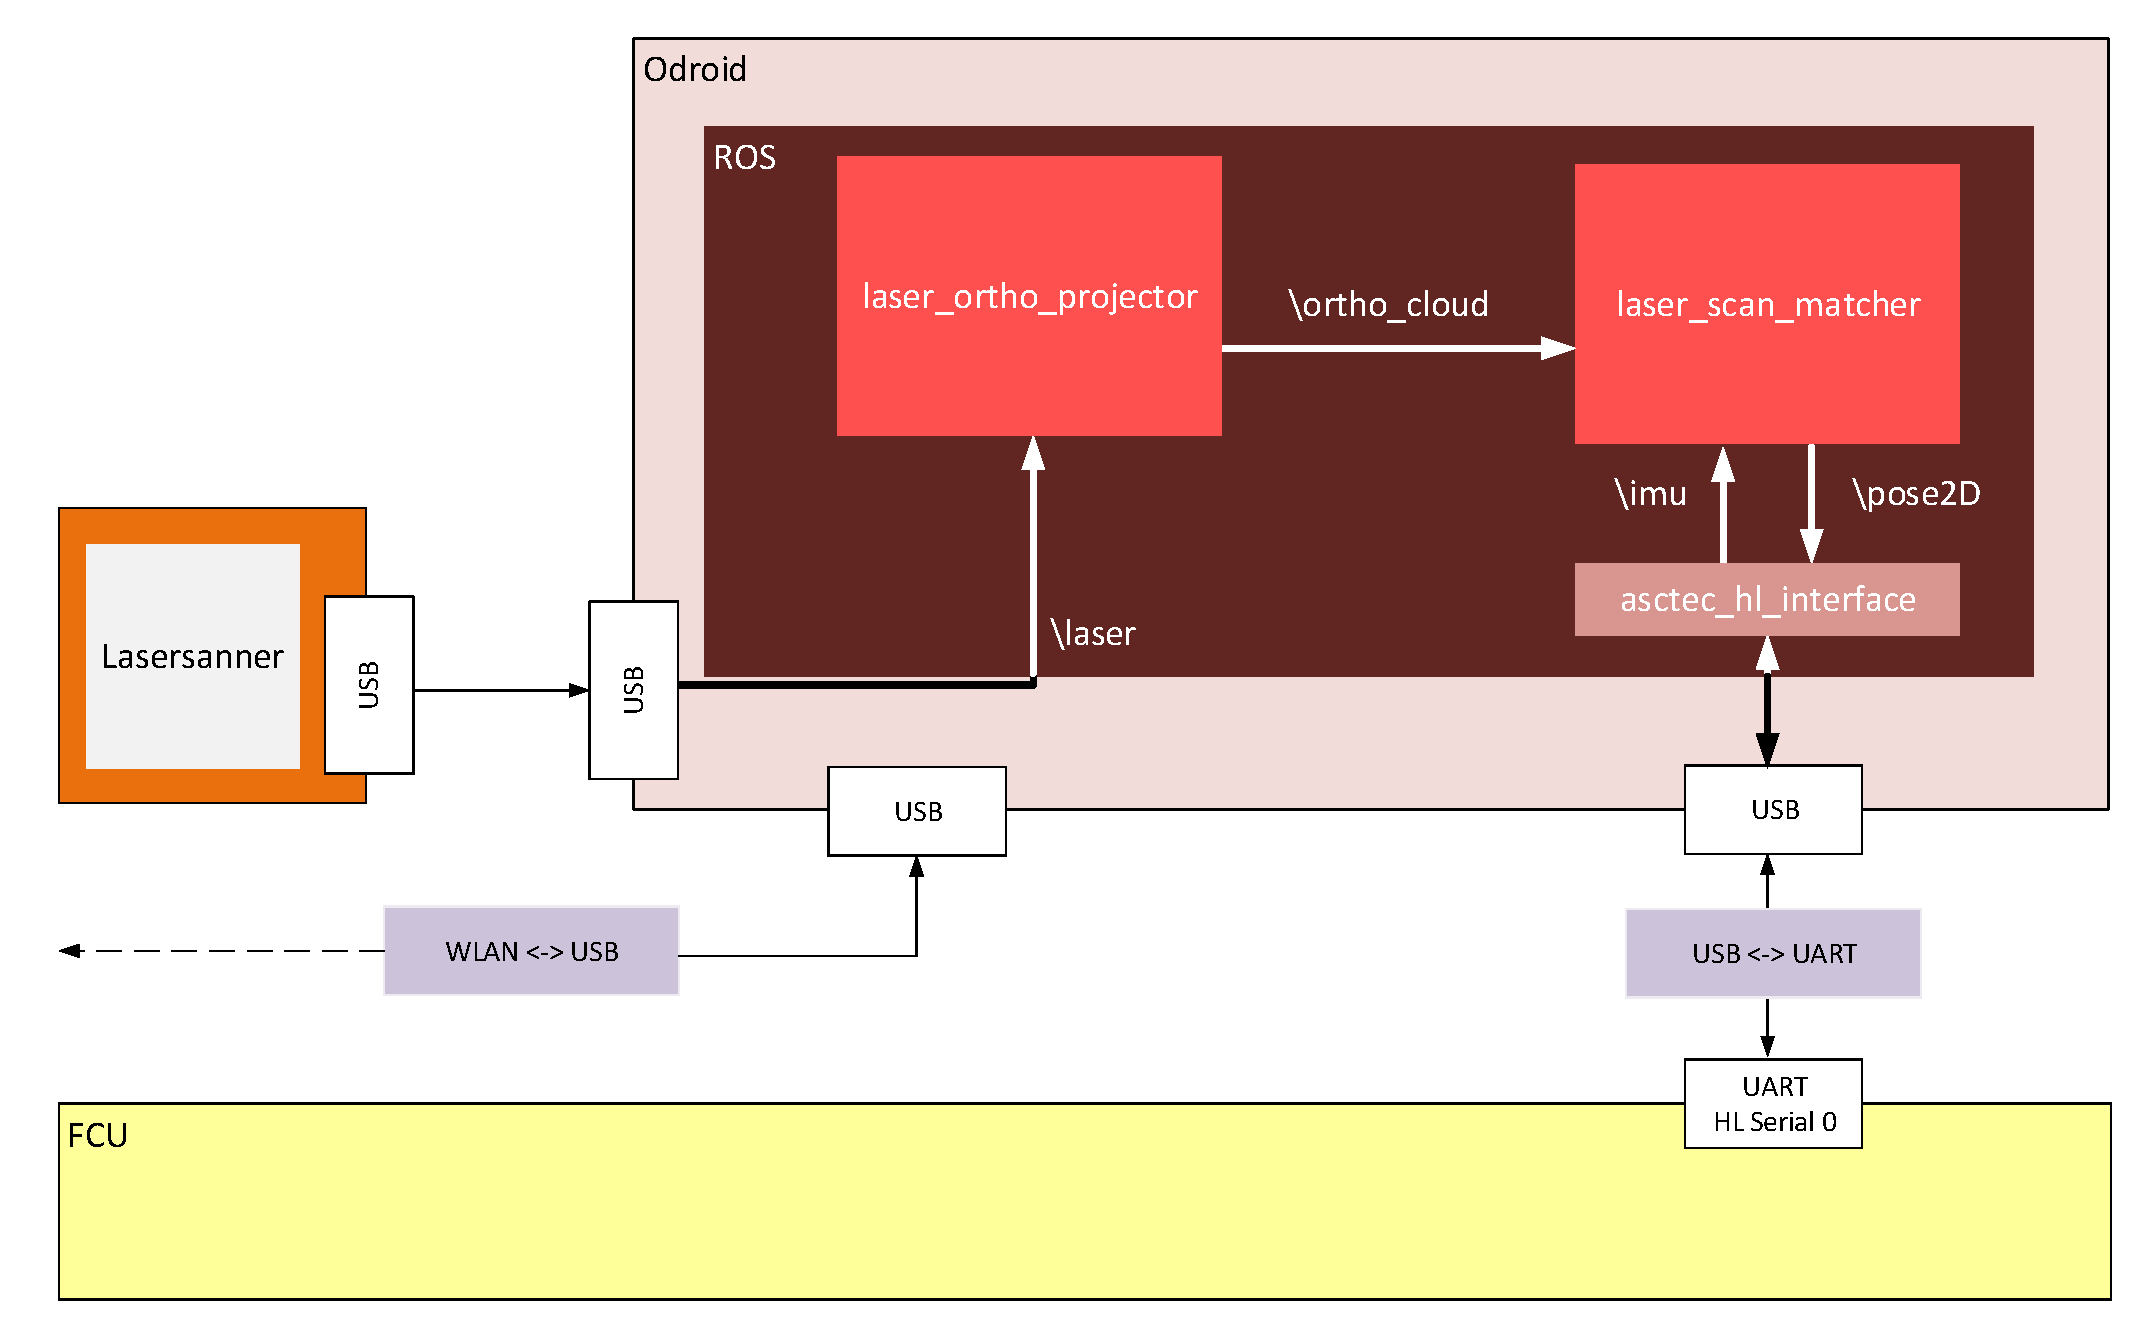
\includegraphics[width = .55\textwidth]{images/ros_ortho_scan_node}
	\caption[Verkn�pfung der Scantools]{Verkn�pfung des \glqq laser\_ortho\_projector \grqq - und des \glqq laser\_scan\_matcher\grqq -Knoten GRAFIK EVENTUELL �BERARBEITEN DA ASCTEC\_HL\_INTERFACE KNOTEN DER F�R DIE KOMMUNIKATION VERANTWORTLICH IST FEHLT} %
	\label{fig:verkn_scantools}
\end{figure}

Realisiert sind diese Vorg�nge in den von \gls{ros} zu Verf�gung gestellte scan\_tools.  Genauer gesagt handelt es sich dabei um dem \glqq laser\_ortho\_projector \grqq - und dem  \glqq laser\_scan\_matcher\grqq -Knoten (Abbildung \ref{fig:verkn_scantools}).Ziel der folgenden Kapitel ist es die Mathematik sowie die Funktionsweise die hinter diesen Algorithmen steht zu erl�utern. 	

ANMERKUNG ES FEHLT NOCH EIN LITERATURVERZEICHNIS!	



\section{Projektion der Laserdaten in das o-frame auf der xy-Ebene des n-frames (\glqq laser\_ortho\_projector\grqq) }
\label{sec:laser_ortho}
Bei der Laserprojektion werden die Laserdaten des l-frame orthogonal zur xy-Ebene des n-frames in die des o-frame transformiert. In allgemeiner Form ist dies in Abbildung \ref{fig:laser_proj_allg} dargestellt. M�glich ist diese Art der Projektion nur unter der Annahme, das es sich bei den erfassten Objekten um Gegenst�nde handelt, die Aufgrund ihrer rechtwinkligen Eigenschaften unabh�ngig der H�he in der sie erfasst werden die gleich Formen aufweisen. In geschlossen R�umen ist diese Annahme zutreffend, da es sich bei den Objekten haupts�chlich um W�nde handelt. Durch Erf�llung dieser Voraussetzungen kann die Flugh�he des Quadrocopters vernachl�ssigt werden. Dies kann man aus Abbildung \ref{fig:laser_proj_pi} entnehmen. Eine Verschiebung des Koordinaten Ursprungs des b-frames auf der z-Achse des o-frames hat demzufolge keinen Einfluss auf die Projektion. Folglich kann f�r beide Koordinatensystem der identischen Ursprung angenommen werden. Unter Beachtung dieser Annahmen wird im Folgenden die Transformation der Laserdaten das o-frame dargestellt.\\

  
\begin{figure}
	
	\centering{
		\subfloat[Allgemeine Projektion der Laserdaten]{
			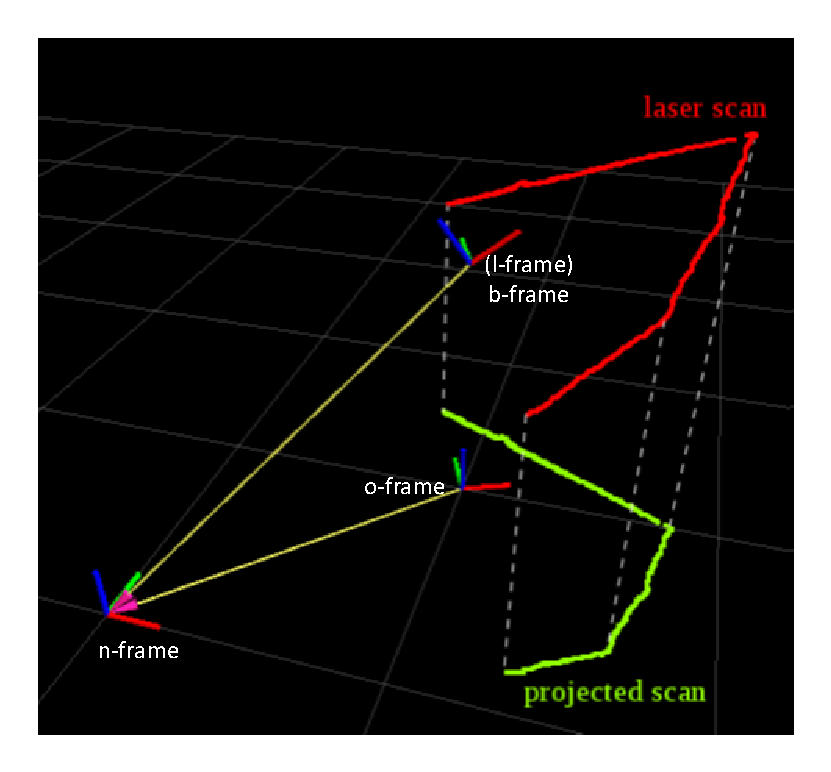
\includegraphics[width=0.5\textwidth]{images/laser_scan_project}
			\label{fig:laser_proj_allg}
		}
		\subfloat[Projektion eines Punkt $P_i$ in den o-frame]{
			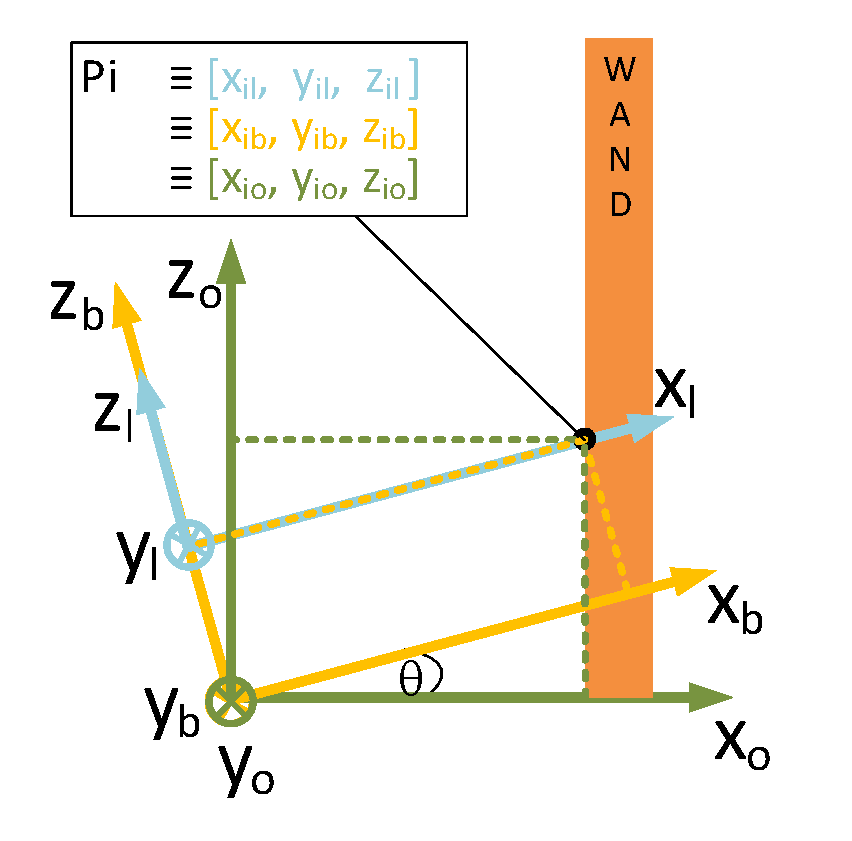
\includegraphics[width=0.5\textwidth]{images/laser_ortho_pro_zx_bsp}
			\label{fig:laser_proj_pi}
		}
	}	
	\caption[Laserprojektion]{Projektion der Laserdaten}
	\label{fig:laser_proj}
	
\end{figure}

Die Entfernungsdaten eines Umlaufs besteht aus mehreren diskreten Abtastungen. �bergeben werden sie in Form von Entfernung $r_i$ in einem Array $r$. Mittels der Schrittweite von $0.25^\circ$ l�sst sich anhand des Indizes $i$ jeder Messung einen Winkel $\gamma$ zuweisen. 
\begin{equation}
\gamma_i = 135^\circ - 0.25^\circ \cdot i
\end{equation}
Die Entfernung eines Punktes $P_i$ ist somit �ber $\{r_i, \gamma_i\}$ definiert. Zur weiteren Verwendung ist es notwendig die Messungen im kartesischen Koordinatensystem des l-frame zu �bertragen.

  \begin{equation}
  P_{il} = 
  \begin{bmatrix}
  \cos(\gamma_i)\cdot r_i, & \sin(\gamma_i)\cdot r_i, & 0
  \end{bmatrix}^T
  \end{equation}
  
Da der Bezugspunkt des o-frames im Schwerpunkt des Quadrocoptes liegen soll, in dem auch der b-frame seinen Ursprung hat, ist es von n�ten die Laserdaten vom l-frame ins b-frame zu transformieren. Wie schon in Kapitel \ref{sec:koordinatensysteme&transformationen} erw�hnt handelt es sich dabei um eine Konstante Transformation. Genauer gesagt um einen Offset von $10cm$ auf der $z^b$-Achse, da der Laser Oberhalb des Quadrocopterschwerpunktes montiert ist.

\begin{equation}
P_{ib} = 
\begin{bmatrix}
\cos(\gamma_i)\cdot r_i, & \sin(\gamma_i)\cdot r_i, & 0,1
\end{bmatrix}^T
\end{equation}
 
 %Bemerkungen:
% keine Rotation um yaw
 %Orientierung der x-Achse identisch da zu erst um y-achse gedreht siehe Konvention
 %Transformationsmatrix auf richtung achten
 %�berpr�fung der berechnung der nein gamma winkel des Lasers. Und Sinn dahinter .Wahrschienlich unn�tz

\begin{figure}
	\centering
	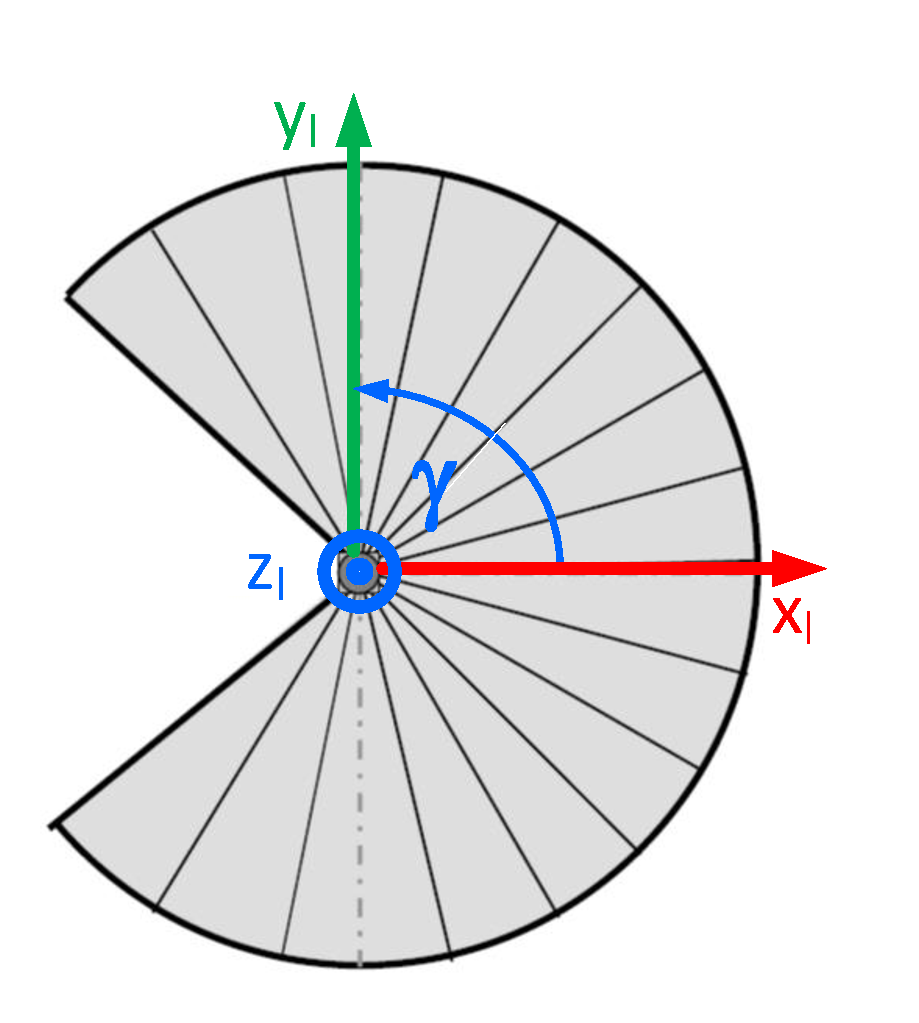
\includegraphics[width = .55\textwidth]{images/l_frame}
	\caption[l-frame]{Draufsicht l-frame} %
	\label{fig:l-frame}
\end{figure}

\section{Positionsbestimmung anhand der ins o-frame �berf�hrten Laserdaten �ber scanmatching}
\label{sec:laser_scan_matching}